\documentclass{fisatprojectfinal}
\title{Pose Estimation Using Deep Learning}
\team{Aman K. Shihab \\ Aneeta Shajan}
\author{Aman K. Shihab}
\regno{FIT19CS015}
\begin{document}
\maketitle
\makecert

\newpage
\pagenumbering{roman}
\setcounter{page}{1}
\newgeometry{top=4cm,bottom=0.1cm}
\thispagestyle{plain}
\renewcommand\abstractname{ABSTRACT}
\begin{abstract}
\vspace{5cm}
Single-person human pose estimation facilitates markerless movement analysis in sports, as well as in clinical applications.
Still, state-of-the-art models for human pose estimation generally do not meet the requirements of real-life applications.
The proliferation of deep learning techniques has resulted in the development of many advanced approaches. However,
with the progresses in the field, more complex and inefficient models have also been introduced, which have caused
tremendous increases in computational demands. To cope with these complexity and inefficiency challenges, we propose
a novel convolutional neural network architecture, called EfficientPose, which exploits recently proposed EfficientNets
in order to deliver efficient and scalable single-person pose estimation. EfficientPose is a family of models harnessing
an effective multi-scale feature extractor and computationally efficient detection blocks using mobile inverted bottleneck
convolutions, while at the same time ensuring that the precision of the pose configurations is still improved. Due to its low
complexity and efficiency, EfficientPose enables real-world applications on edge devices by limiting the memory footprint
and computational cost. The results from our experiments, using the challenging MPII single-person benchmark, show that
the proposed EfficientPose models substantially outperform the widely-used OpenPose model both in terms of accuracy and
computational efficiency. In particular, our top-performing model achieves state-of-the-art accuracy on single-person MPII,
with low-complexity ConvNets.
\end{abstract}



\newpage
\renewcommand\abstractname{Contribution by Author}
\thispagestyle{plain}
\begin{abstract}
\vspace{5cm}
Author Contribution  Goes Here
\vspace{1cm}
\begin{flushright}
Student Name
\end{flushright}
\end{abstract}

\newpage
\renewcommand\abstractname{ACKNOWLEDGEMENT}
\thispagestyle{plain}
\begin{abstract}
\vspace{5cm}
Your Acknowledgement Goes Here
\vspace{1cm}
\begin{flushright}
Student 1
\end{flushright}
\end{abstract}
\newpage

\restoregeometry
\tableofcontents
\thispagestyle{plain}
\newpage

\cleardoublepage
\addcontentsline{toc}{chapter}{\listfigurename}
\listoffigures
\newpage

\cleardoublepage
\addcontentsline{toc}{chapter}{\listtablename}
\listoftables
\newpage



\chapter{Introduction}
\pagenumbering{arabic}
\setcounter{page}{1}
\renewcommand{\baselinestretch}{1.50}
\section{Overview}
Single-person human pose estimation (HPE) refers to the
computer vision task of localizing human skeletal keypoints
of a person from an image or video frames. Single-
person HPE has many real-world applications, ranging from
outdoor activity recognition and computer animation to clinical assessments of motor repertoire and skill practice
among professional athletes. The proliferation of deep
convolutional neural networks (ConvNets) has advanced
HPE and further widen its application areas. ConvNet-based
HPE with its increasingly complex network structures,
combined with transfer learning, is a very challenging task.
However, the availability of high-performing ImageNet
backbones, together with large tailor-made datasets, such
as MPII for 2D pose estimation, has facilitated the
development of new improved methods to address the
challenges.
\begin{figure}[h!]
\begin{center}
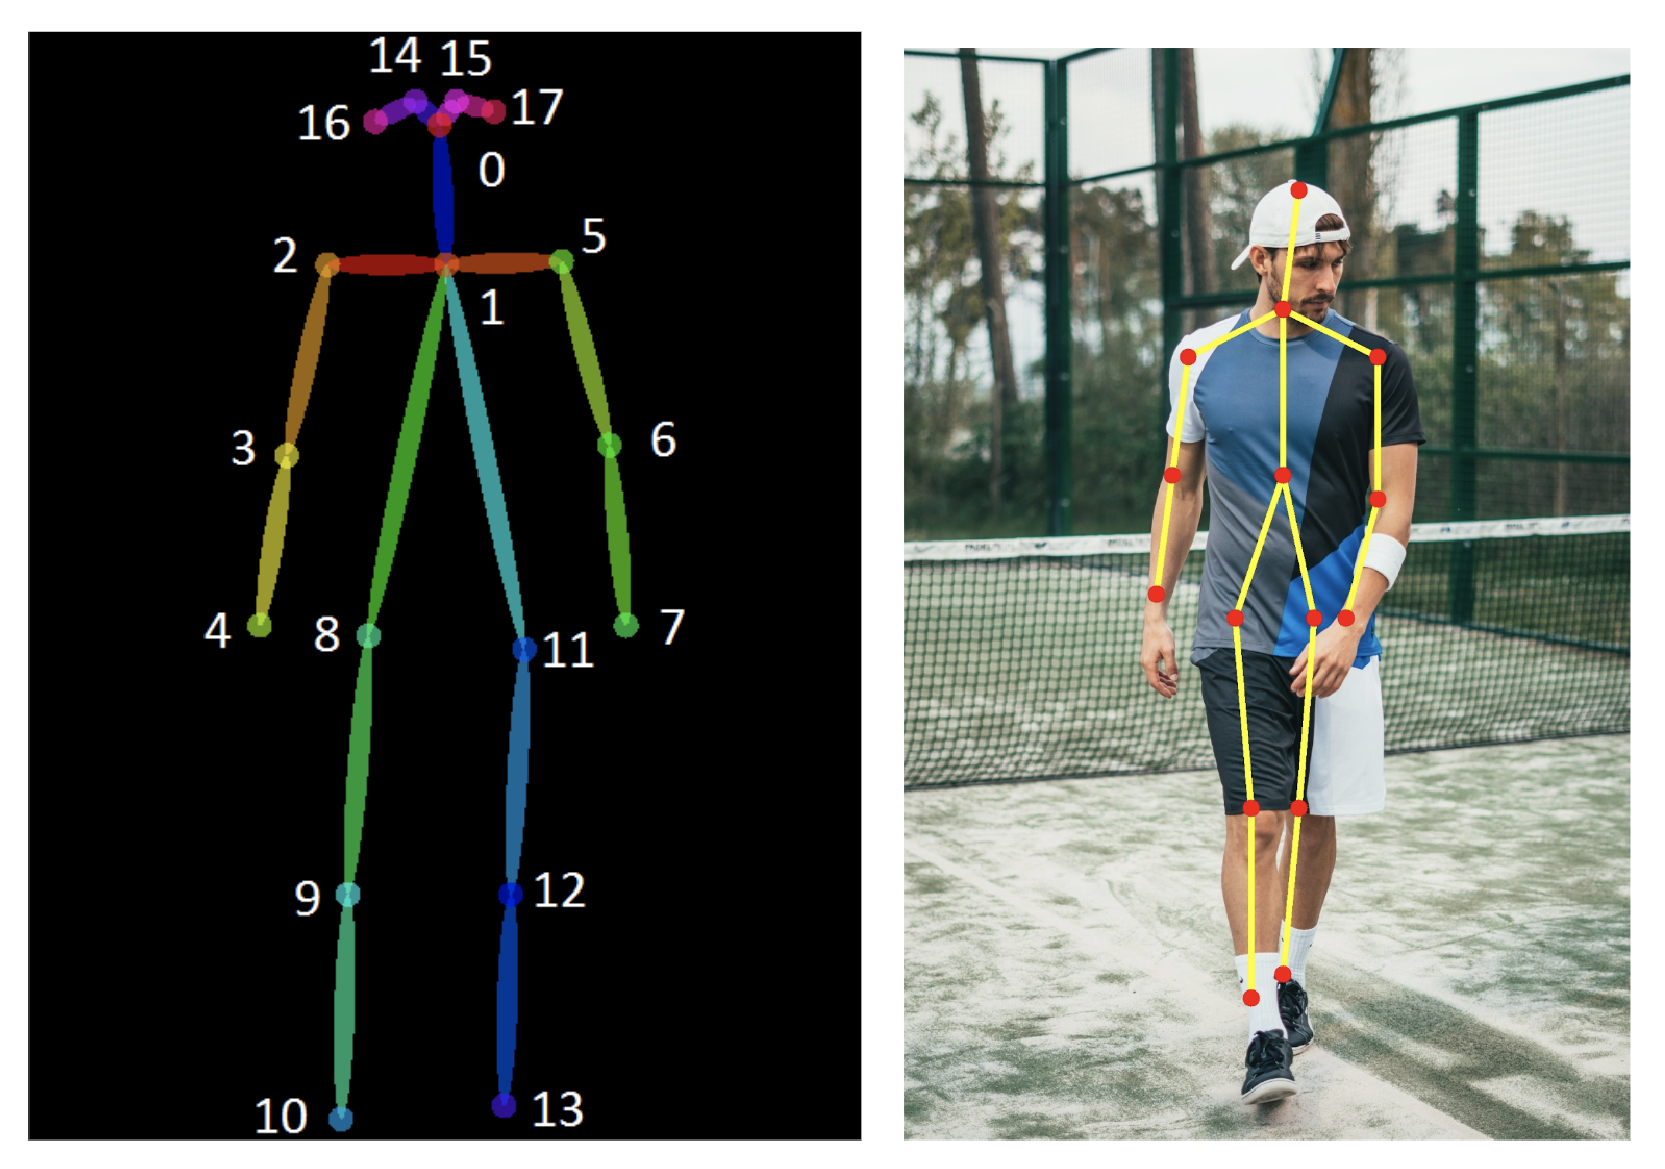
\includegraphics[scale=.3]{pose-estimation}
\caption{Human Pose Estimation Demo}
\end{center}
\end{figure}
An increasing trend in computer vision has driven towards
more efficient models. Recently, Efficient-
Net was released as a scalable ConvNet architecture,
setting benchmark record on ImageNet with a more com-
putationally efficient architecture. 
\section{Problem Statement}

Despite the availability of more performant, efficient layers and architecture's, it has not quite transalated
into fruitful results within human pose estimation, there is still a lack of architectures that
are both accurate and computationally efficient at the same
time. In general, current state-of-the-art architectures are
computationally expensive and highly complex, thus making them hard to replicate, cumbersome to optimize, and
impractical to embed into real-world applications. \par

Minimal and efficient model architectures are coveted for their ability to run on edge devices with minimal hardware requirements.
This also greatly reduces the response times thereby becoming increasingly relevant for real-time applications.
The ability to run real-time is a crucial feature for pose estimation, because often times in most applications it's desirable to obtain the outputs instantly to judge the output.

\section{Objective}

Primary objective is to exploit recent advances in ConvNets and shed some light onto
an improved approach called EfficientPose. The main idea
is to modify OpenPose, a well-known pose estimation model into a family of scalable ConvNets
for high-precision and computationally efficient single-person
pose estimation from 2D images. 
Then we evaluate the EfficientPose model by comparing
it against the original OpenPose model on single-person
HPE. After that, we compare it against the current state-of-
the-art single-person HPE methods on the official MPII
challenge, focusing on accuracy as a function of the number
of parameters. EfficientPose models aim to
elicit high computational efficiency, while bridging the gap
in availability of high-precision HPE networks.

\chapter{Related works}

Ever since the increased adoption of ConvNets for HPE following the
success of DeepPose has set the path for accurate HPE.
Another breakthrough in HPE was provided by OpenPose. OpenPose comprises a multi-
stage architecture performing a series of detection passes.
Provided an input image of 368 × 368 pixels, OpenPose
utilizes an ImageNet pretrained VGG-19 backbone to
extract basic features. The features are
supplied to a DenseNet-inspired detection block
arranged as five dense blocks, each containing three 3×
3 convolutions with PReLU activations. The detection
blocks are stacked in a sequence. First, four passes of part affinity fields map the associations
between body keypoints. Subsequently, two detection
passes predict keypoint heatmaps to
obtain refined keypoint coordinate estimates. In terms of
level of detail in the keypoint coordinates, OpenPose is
restricted by its output resolution of 46 × 46 pixels.
The OpenPose architecture can be improved by recent
advancements in ConvNets, as follows: First, automated
network architecture search has found backbones that are more precise and efficient in image
classification than VGG and ResNets. Compound model scaling can
balance the image resolution, width (number of networkchannels), and depth (number of network layers). This
resulted in scalable convolutional neural networks, called
EfficientNets, with which the main goal was to provide
lightweight models with a sensible trade-off between model
complexity and accuracy across various computational
budgets. For each model variant EfficientNet, from the
most computationally efficient one being EfficientNet-B0
to the most accurate model, EfficientNet-B7.The total no. of FLOPS increases by a factor of 2, given by:
	
	$$
	(\alpha. \beta^2. \gamma ^ 2) ^ \phi
	$$
where $$ \alpha = 1.2 , \beta = 1.1, \gamma = 1.15 $$
They denote the coefficients for depth, width and resolution respectively.
% \begin{table}[h!]
% \begin{center}
% 	\caption{World Population Table} 
% \begin{tabular}{|c|c|c|c|}
	
% \hline Rank & Country & Population  & Percentage  \\ 
% \hline 1 & China & 1,347,350,000 & 19.24\% \\ 
% \hline 2 & India & 1,210,193,422  & 17.28\% \\ 
% \hline 3 & United States & 313,269,000 & 4.47\% \\ 
% \hline 
% \end{tabular}
% %\caption{World Population Table} 
% \end{center}
% \end{table}
\begin{figure}[h!]
	\begin{center}
	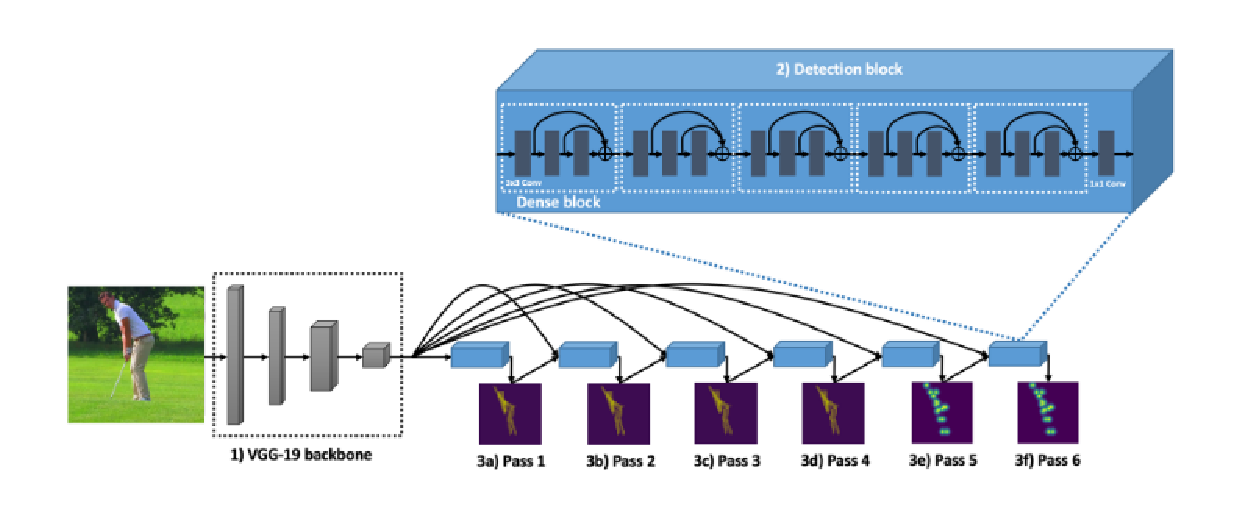
\includegraphics[scale=.8]{OpenPose}
	\caption{OpenPose}
	\end{center}
	\end{figure}
\par
Second, parallel multi-scale feature extraction has improved
the precision levels in HPE, emphasizing
both high spatial resolution and low-scale semantics.
However, existing multi-scale approaches in HPE are
computationally expensive, both due to their large size and
high computational requirements. For example, a typical
multi-scale HPE approach has often a size of 16 to 58
million parameters and requires 10 to 128 GFLOPS. To cope with this, we propose cross-
resolution features, operating on high- and low-resolution
input images, to integrate features from multiple abstraction
levels with low overhead in network complexity and with
high computational efficiency. Existing works on Siamese
ConvNets have been promising in utilizing parallel network
backbones. Third, mobile inverted bottleneck
convolution (MBConv) with built-in squeeze-and-
excitation (SE) and Swish activation integrated
in EfficientNets has proven more accurate in image
classification tasks than regular convolutions, while substantially reducing the computational costs. The efficiency of MBConv modules stem from
the depthwise convolutions operating in a channel-wise
manner. With this approach, it is possible to reduce the
computational cost by a factor proportional to the number
of channels. Hence, by replacing the regular 3 × 3
convolutions with up to 384 input channels in the detection
blocks of OpenPose with MBConvs, we can obtain more
computationally efficient detection blocks. Further, SE
selectively emphasizes discriminative image features,
which may reduce the required number of convolutions and
detection passes by providing a global perspective on the
estimation task at all times. Using MBConv with SE may
have the potential to decrease the number of dense blocks
in OpenPose. Fourth, transposed convolutions with bilinear
kernel scale up the low-resolution feature maps, thus
enabling a higher level of detail in the output confidence
maps.The main advantage
of this is that we can use ConvNets that are small and
computationally efficient enough to run on edge devices
with little memory and low processing power, which is
impossible with OpenPose.


\chapter{Design}

\section{Introduction}
Here, the model architecture we use, namely EfficientPose exploits the recent advancements in ConvNets
and additionally concatenates high-level and low-level features. The net result is a much more efficient model
with better accuracy and needing fewer computaional resources.

\section{Architecture}

\begin{figure}[h!]
	\begin{center}
	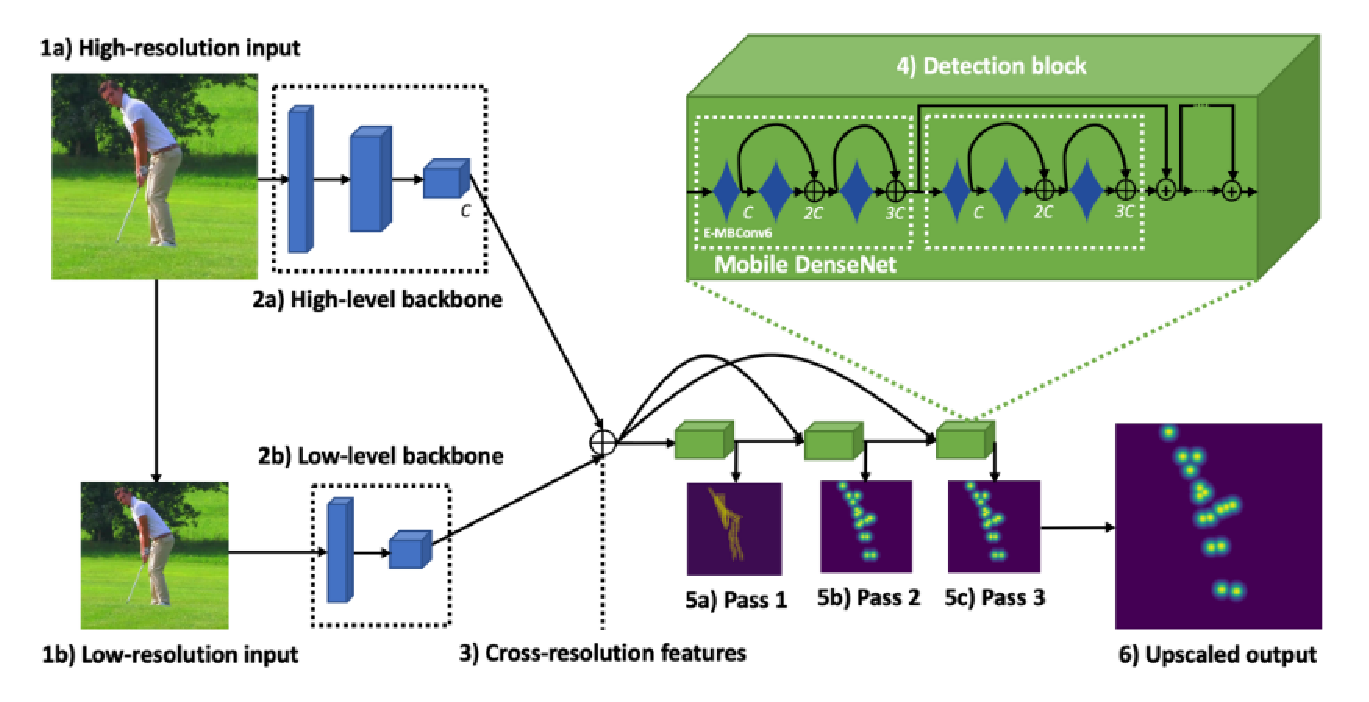
\includegraphics[scale=0.6]{EfficientPose}
	\caption{EfficientPose}
\end{center}
\end{figure}

The model takes in two inputs, one is the high-level features and second is the low-level features.
The low level features are obtained by downsampling an image to half of it's height and width using an average pooling layer.
The feature extractors here are initial layers of EfficientNet. For high level extractor, $\phi \in [0,7]$ and 
for the low level extractor $\phi \in [0,3]$.
\par
These extracted features and then concatendated together to obtain cross-resolution features.
This helps us to emphasize the important local factors in the image of interest.
\par
The input to the next phase of the model is the cross-resolution features obtained in the previous step.
Here the required keypoints are localized through an iterative process, where each
detection pass performs supervised prediction of output maps.
Each detection pass comprises a detection block
and a single 1 × 1 convolution for output prediction.
The detection blocks across all detection passes exhibit the
same basic architecture, comprising Mobile DenseNets.
Data from here is forwarded to the successive layers through skip connections.
Here, we also avoid downsampling of the output to preserve the resolution.
The original mobile convnets are modified by adding an E-swish activation function with $\beta$ value 1.25.
\par
The overall detection is performed in two rounds. Initially, the overall pose of the person is anticipated through a single pass of skeleton estimation. This helps especially when
there are multiple people present in the frame.
After the skeleton estimation is done two detection passes are performed to estimate heatmaps for points of interest.

\par
Another improvement on top of OpenPose is that, EfficientPose projects lower-resoltion image onto a higher resolution space using transposed convolution to allow an increased level of detail, whereas in OpenPose the heatmaps are
constrained to the lower space.
\section{Design of modules}
In mathematics, Stirling's approximation (or Stirling's formula) is an approximation for large factorials. It is named after James Stirling.

\chapter{Results}

Compiled languages arelanguages typically processed by compilers, though theoretically any language can be compiled or interpreted. The important ones are:
\begin{itemize}
\item Ada
\item C
\item C++
\item Fortran
\item Java
\end{itemize}




\chapter{Conclusion}

An intrusion detection system (IDS) \cite{nist} is a device or software application that monitors network and/or system activities for malicious activities or policy violations and produces reports to a Management Station.


Donald Ervin Knuth \cite{knuth} is a computer scientist and Professor Emeritus at Stanford University. He is the author of the seminal multi-volume work The Art of Computer Programming. Knuth has been called the "father" of the analysis of algorithms


\begin{thebibliography}{1}
\bibitem{nist} K. Scarfone and P. Mell, ``Guide to intrusion detection and prevention systems
(idps),'' \textit{NIST Special Publication}, vol. 800, no. 2007, p. 94, 2007.
\bibitem{knuth} Wikipedia, ``Donald knuth.'' \url{http://en.wikipedia.org/wiki/Donald_Knuth}.
\end{thebibliography}

\begin{appendices}
Test
\end{appendices}


\end{document}
